\documentclass{article}
\usepackage{graphicx} % For including images
\usepackage[table,xcdraw]{xcolor} % For table coloring (optional)
\usepackage{caption} % For controlling captions

% Define row colors for different turns
\usepackage{colortbl} % For row coloring
\usepackage{lipsum}   % Optional: For generating filler text

% Define custom colors for near-white shades
\usepackage{tcolorbox}
\usepackage{lscape}

\begin{document}

\begin{table}[ht]
\centering
\begin{tabular}{|c|c|l|}
\hline
\textbf{} & \textbf{Turn} & \textbf{Description} \\
\hline
\rowcolor{gray!10} 
\includegraphics[scale=0.07]{figs/emojis/emoji_1.png} & 0 & Win Condition Recognition \\
\hline
\rowcolor{gray!10} 
\includegraphics[scale=0.07]{figs/emojis/emoji_2.png} & 0 & Rule Modification \\
\hline
\rowcolor{gray!10} 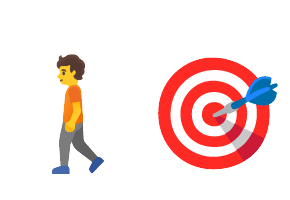
\includegraphics[scale=0.07]{figs/emojis/emoji_3.png} & 0 & Direct Navigation Efficiency \\
\hline
\rowcolor{gray!10} 
\includegraphics[scale=0.07]{figs/emojis/emoji_4.png} & 0 & Context-Sensitive Decision Making \\
\hline
\rowcolor{gray!30} 
\includegraphics[scale=0.07]{figs/emojis/emoji_5.png} & 1 & Win Rule Construction \\
\hline
\rowcolor{gray!30} 
\includegraphics[scale=0.07]{figs/emojis/emoji_6.png} & 1 & Selective Interaction With Relevant Objects  \\
\hline
\rowcolor{gray!30} 
\includegraphics[scale=0.07]{figs/emojis/emoji_7.png} & 1 & Rule Manipulation and Execution  \\
\hline
\rowcolor{gray!60} 
\includegraphics[scale=0.07]{figs/emojis/emoji_8.png} & 2 & Subtask Coordination \\
\hline
\rowcolor{gray!90} 
\includegraphics[scale=0.07]{figs/emojis/emoji_9.png} & 3 & Immovable Interaction \\
\hline
\end{tabular}
\caption{Metrics and Turn of Introduction for baba-is-ai}
\end{table}

\end{document}
